\chapter{Method}

\section{Data Collection}
\label{sec:data}
The experiment was hosted through an open-source crowdsourcing client/system server system LingoTurk \cite{lingoturk}.
While the participants were recruited via Prolific \cite{prolific} - a subject pool for online experiments. The following criteria were used to filter the participants: native English speaker located in the UK, age in range 18-40, minimal approval rate of 95\%, number of previous submissions must be ar least 20 studies, participants cannot have taken part in any of the related studies our group has conducted before. The estimated length of the experiment was 22 minutes, while the actual median was 19 minutes 30 seconds. The participants were paid 3.89 pounds which is equivalent to minimal hour wage in Germany. The participants were paid only in case of successful completion of the full experiment. The experiment was conducted in a web browser and the participants were asked to use a computer with functional webcam. 


\subsection{Reference Games}
\label{sec:data:ref_games}
There are 3 conditions of the reference games: Simple, Complex and Unambiguous. In the \autoref{sec:rsa} we mainly talked about the Simple and Complex conditions. The Unambiguous condition suits two main purposes. First of all, it acts as a sort of filler, so that participants do not get used to the same type of problems. Second of all, it acts as a control check, that is, participants who do not reach over 50\% accuracy on the Unambiguous trials are excluded from the analysis.

The trials were generated using 3 colors: red, green and blue, and 3 shapes: square, circle and triangle. In total there are 72 combinations of unique trials. The full list of trials can be found \TODO{insert link to apendix}. The code used to generate trials can be found at \TODO{insert link to the source code} For each condition every unique sent message was repeated exactly twice. Which results in 12 trials of every condition. Furthermore one simple and one complex trial was picked to be repeated once again in the very end of the experiment. These were so called strategy trials where we would ask the participants to explain their reasoning behind the choice of the object. All trials were randomly shuffled before the experiment, except for the strategy trials which were always at the end of the experiment.

\begin{figure}
    \centering
    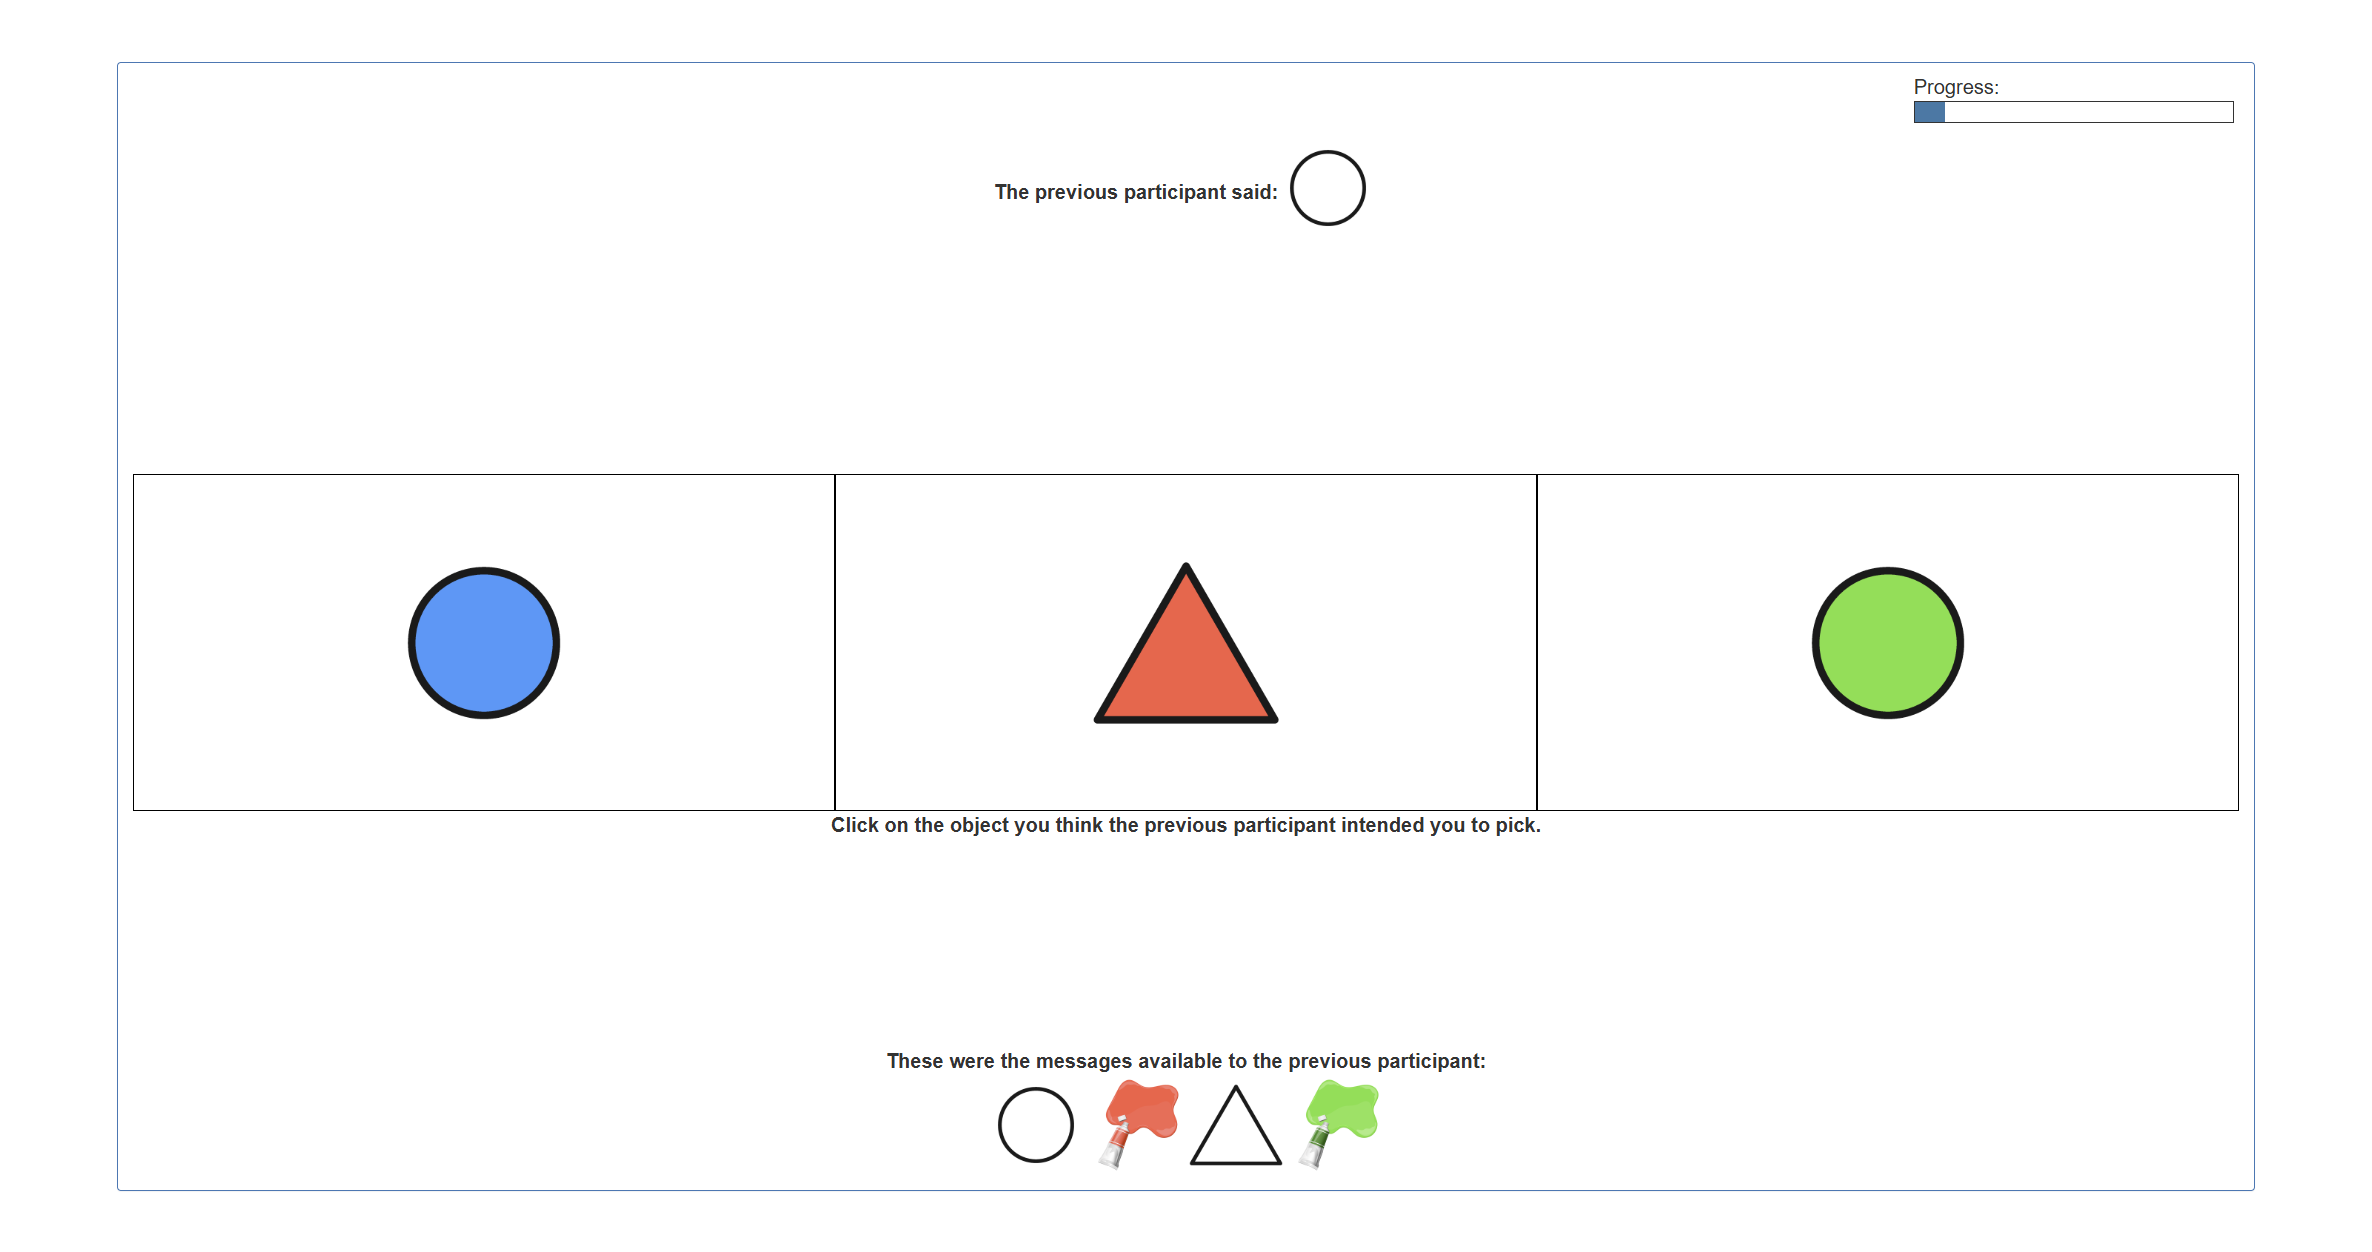
\includegraphics[width=0.8\textwidth]{images/example_trial.png}
    \caption{Example trial}
    \label{fig:example_trial}
\end{figure}

Before the main part of the experiment with 36 + 2 trials, the participants were asked to do a speaker's job in reference games with 3 Unambiguous trials and 1 completely ambiguous one. The participants were asked to describe the object in the ambiguous trial in a way that the listener would be able to pick the correct object. Later they were told that a previous participant had already done the speaker's job and they were to do the listener's job, which was the main part of the experiment with 36 + 2 trials. An example trial can be seen in \autoref{fig:example_trial}.

\subsection{Eye Tracking}
\label{sec:data:eyetr}
The eye tracking was done via library \cite{wegbazer}. The library was used to track participants' gaze on the screen. There was a calibration in the beginning of the experiment after the practice trials where participants did the speaker's job, this allowed to put the calibration as close to the main experiment as possible. The calibration was adapted from the one used in the demo of \cite{wegbazer}. Although, we included 11 points instead of 9, the additional points were put on the objects' places. Each point had to be clicked 5 times. In addition, the calibration accuracy assessment in the end was done not with 1 point but 3: middle, left and right. Where left and right again correspond to the positions of the main objects on the screen. 

In order to successfully pass the calibration assessment, the participants must reach at least 65\% accuracy on each of the three calibration points. However, during the testing phase we noticed that the calibration assessment was too strict and difficult to pass. Therefore, it was decided to make the left and right points easier to calibrate via adjusting the calculation of the accuracy. A weighted accuracy calibration procedure was implemented. While the distance between for the accuracy of the middle point was calculated via euclidean distance, the left and right points were calculated via the following formula: $\sqrt{(w_x\cdot(calib\_point\_x - gaze\_x))^2 + (w_y\cdot(calib\_point\_y - gaze\_y))^2}$. Where $w_x$ and $w_y$ are the coefficients that were adjusted during the testing phase. The final values were $w_x = 1$ and $w_y = 0.5$. The values were chosen based on the fact that left and right objects do not have any other objects on the vertical axes this can be seen in \autoref{fig:example_trial}. Therefore a slightly inaccurate result on the vertical axes would be relatively easy to correct during the analysis.

The images were located on the screen as far as possible to reduce the errors as much as possible. For the same reason, the sent message were kept as a single block instead of being spread further apart. 

Furthermore, a performance issue arised during the pilot phase. The issues was that the eye tracking became very slow and laggy towards the end of the second half of the experiment. The more clicks were made, the worse the performance became. The issue was resolved by reducing the \text{DataWindow} size from 700 to 50 in source code and recreating the webgazer source file afterwards.

\section{Analysis}
\label{sec:analysis}

\subsection{Pairwise Correlations}
\label{sec:analysis:corr}

\subsection{Mixed Effects Logistic Regressions}
\label{sec:analysis:mixed_effects}

\subsection{Exploratory Analysis}
\label{sec:analysis:exploratory}

\subsubsection{Clustering}
\label{sec:analysis:exploratory:clustering}

\subsubsection{CNNs}
\label{sec:analysis:exploratory:cnn}
